\subsection{Value functions in belief wealth space}\label{ssec:val-func}

First, we look at action-value functions found by using different utility functions in ~\autoref{fig:val-func}.
As described in ~\autoref{sec:methods} the augmented state space encodes the wealth and the belief of the agent.
The policy is the action with maximum return for each belief wealth pair and is depicted with the blue (waiting) and the orange (selling) dots.
For example, in the very first plot, the agent always sells at 0.8 belief for any wealth value. We call this line the belief threshold.

\begin{figure}[h]
    \centering
    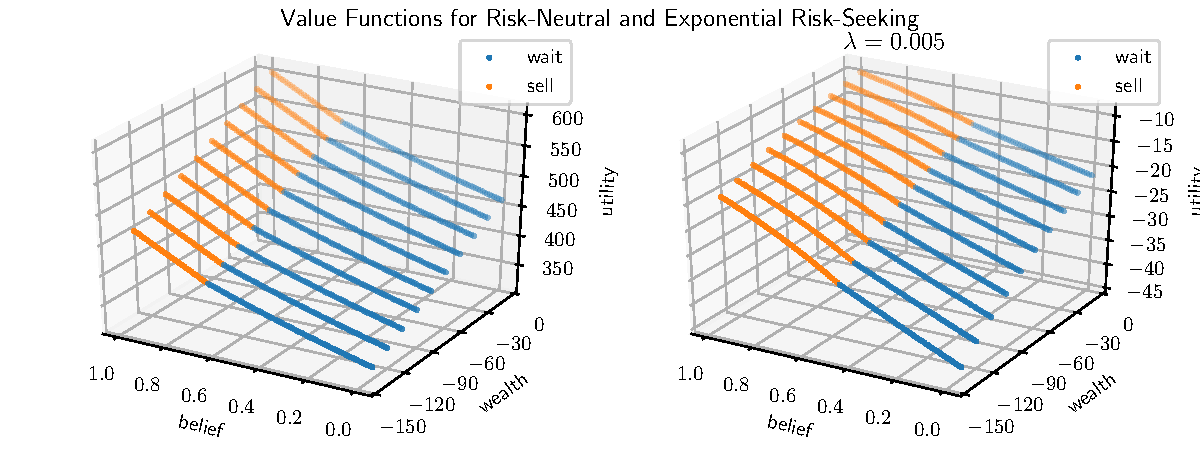
\includegraphics[width=0.99\linewidth]{img/exp_policy.pdf}\\
    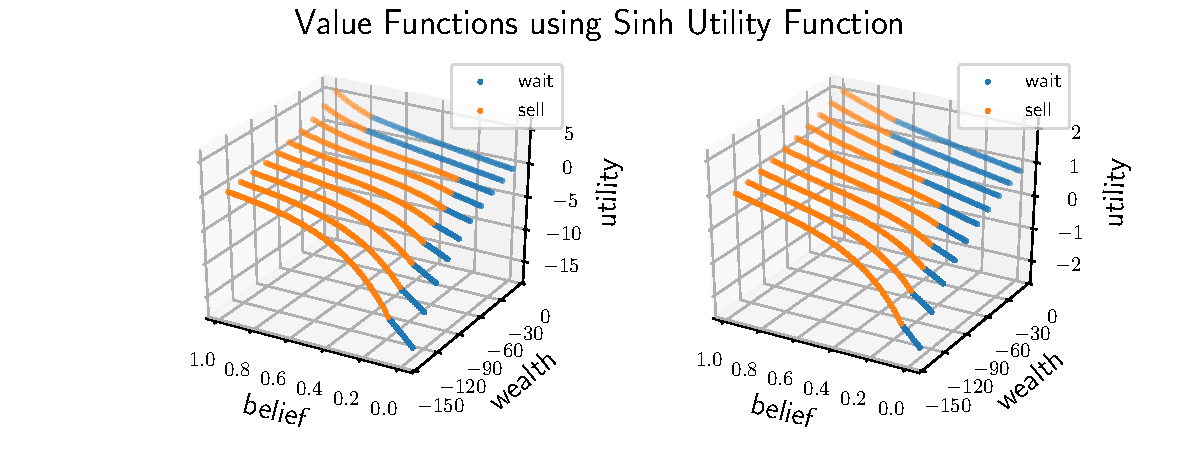
\includegraphics[width=0.99\linewidth]{img/sinh_policy.pdf}\\
    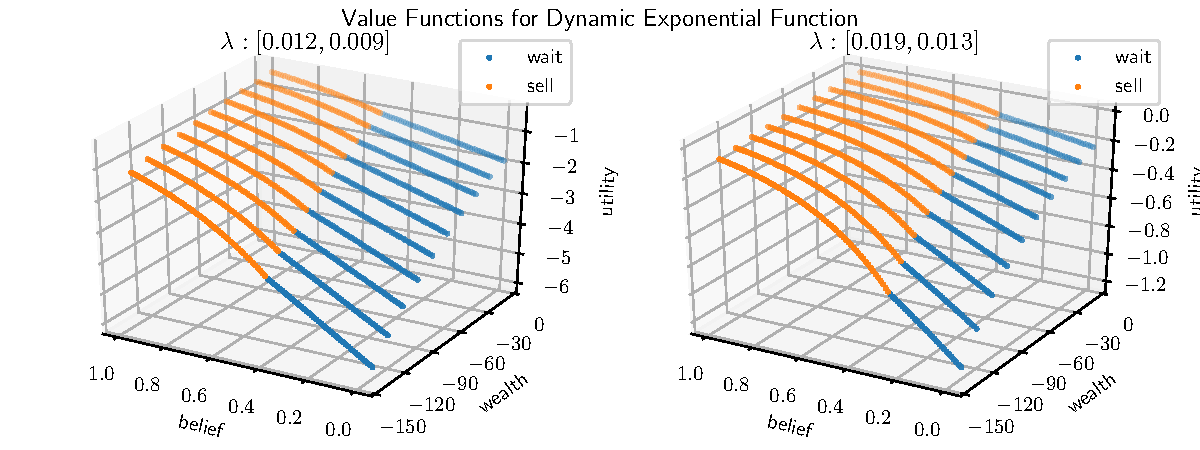
\includegraphics[width=0.99\linewidth]{img/dyn_policy.pdf}
    \caption{Value functions exhibiting different risk-behaviors; from top left: risk-neutral agent (utility function is the identity function), risk-averse agent with exponential utility function, two fixed time agents with different time thresholds, two agents with dynamic exponential utility function.}\label{fig:val-func}
\end{figure}

In the first row, we present value functions that are found by using the risk-neutral (identity function) UF and an exponential UF. Both functions result in agents simply selling above a certain belief threshold, regardless of the current wealth.
The Exponential UF sets this threshold with the $\lambda$ parameter, which is displayed above the plot.
A positive $\lambda$ induces risk-averse behavior, which results in selling with higher belief than the risk-neutral agent.

The second row shows policies derived by the $\text{sinh}$ UF as explained in ~\autoref{equ:sinh}. As opposed to the previous policies they are clearly time-dependent.
The first plot shows what we call a fixed time policy, where the belief threshold for selling decreases abruptly at a specific wealth value (i.e. time).
The second plot shows a similar policy but with a smoother decrease in belief threshold over the wealth axis.

Lastly, in the third row we present the dynamic utility function as explained in ~\autoref{equ:dynexp}.
We selected $\lambda_w$ depending on time by using the simple identity:

\begin{align*}
\text{time} = \frac{\text{wealth}}{\text{observation\ cost}}
\end{align*}

Using this identity, we selected $\lambda_w$ from a logarithmically spaced sequence.
The sequence range is displayed above each plot.
The dynamic utility function was hard to parametrize because most picks for $\lambda_w$ made the resulting function unstable.
Furthermore, it is difficult to perform a grid search due to vast amount of free parameters (possibly as many as time steps).

\begin{figure}[h]
    \centering
    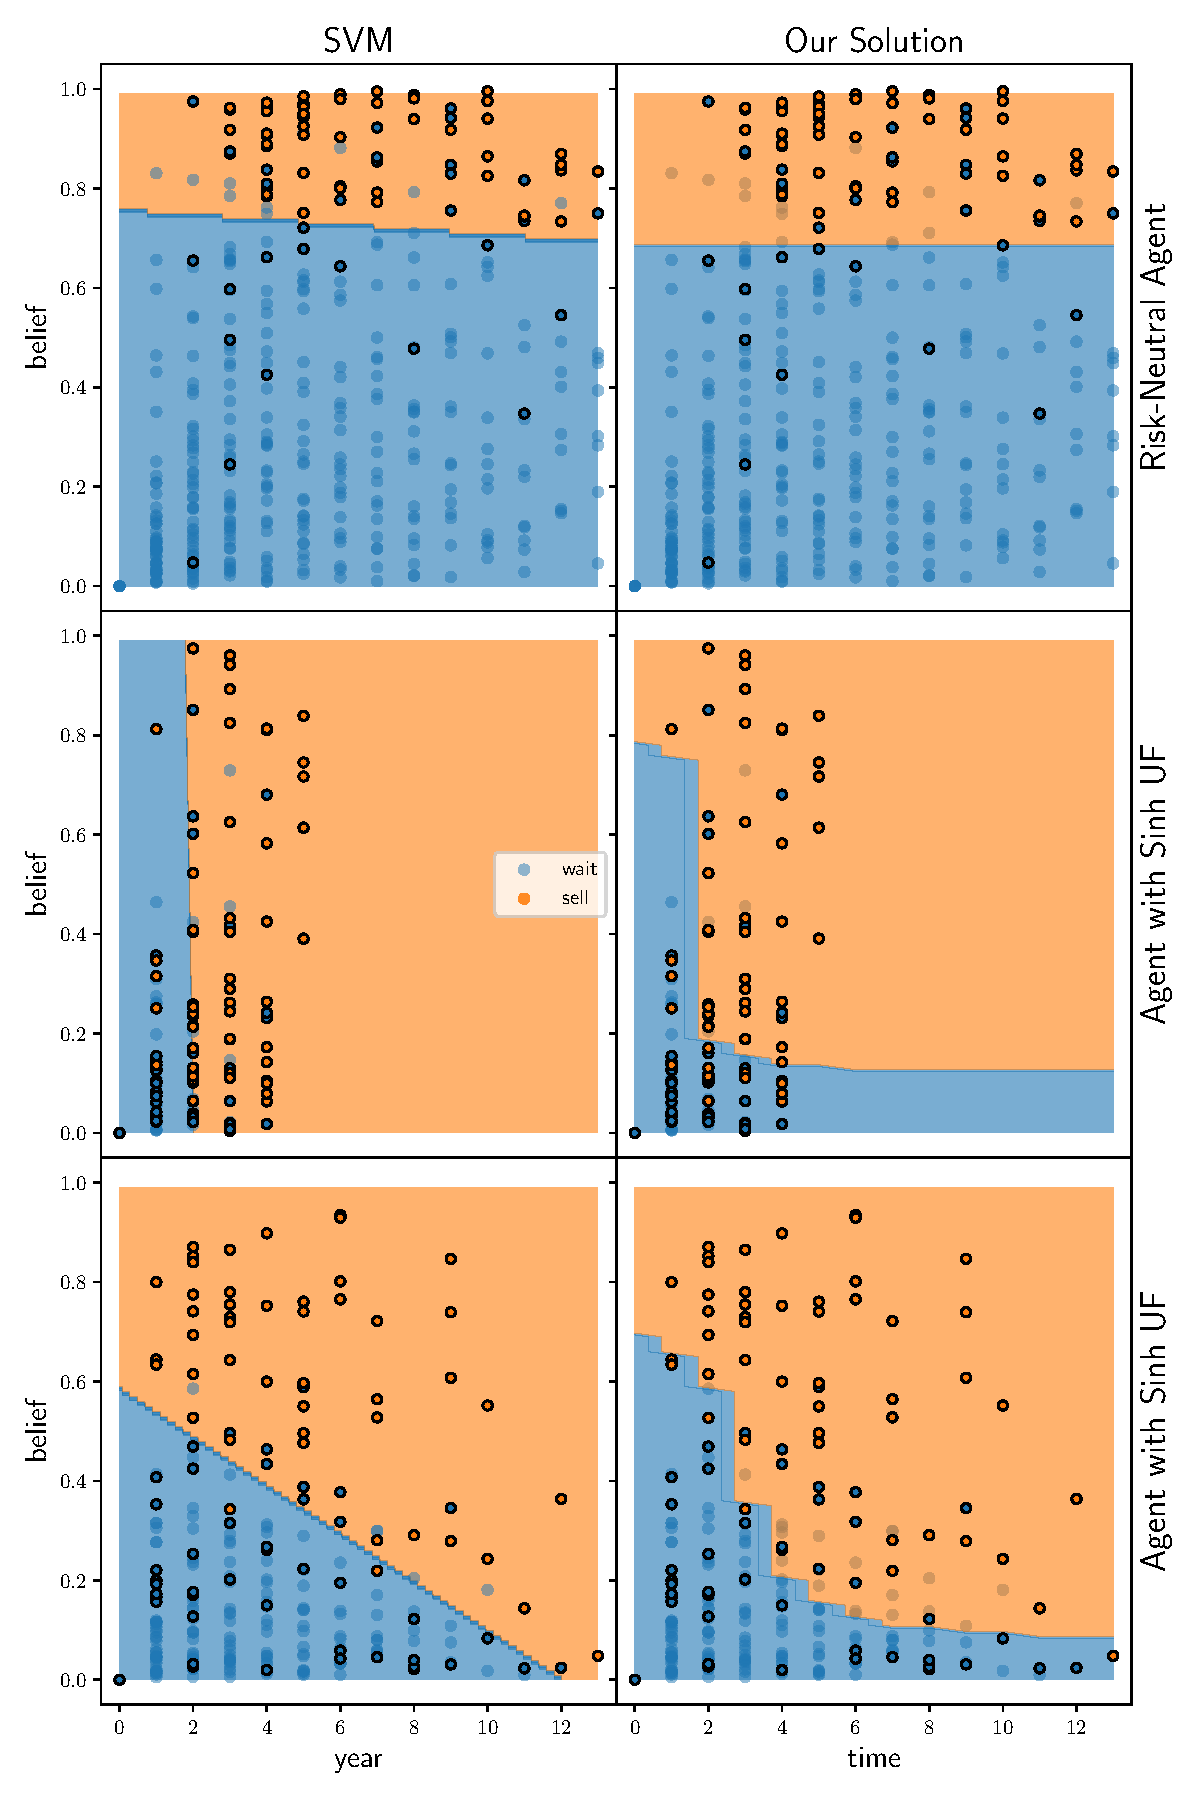
\includegraphics[width=0.99\linewidth]{img/fit}
    \caption{Examples from three distinct human behaviors observed and reproduced with RL agents. Behaviors by row: 1) Constant belief threshold, modeled by the risk-averse exponential utility function, 2) Fixed time threshold, modeled by $\sinh$ utility, 3) Mixed strategy, modeled by $\text{sinh}$ UF. The left column shows the empirical optimal split of data using a linear kernel support vector machine (with cross-validation). The right column shows the optimal policy that is closest to the SVM split, found via grid-search.}
    \label{fig:svm_vs_value}
\end{figure}

\subsection{From human behavior to utility functions}\label{ssec:human-behavior}

In~\autoref{ssec:val-func}, we presented how different utility functions result in different policies.
Now we look at how to derive utility functions and the corresponding risk parameters for the behavioral data from Scenario 2 of the experiment.

In the behavioral data, we distinguished three kinds of behaviors: 1) people selling at a specific belief threshold, 2) people selling at a specific wealth, and 3) people lowering their threshold with decreasing wealth.
We show an example for each of these behaviors in each row of~\autoref{fig:svm_vs_value}.
For each time step (i.e. year) of each trial, we have a data point with the action subject took, the belief shown to the user and the year. These are plotted in~\autoref{fig:svm_vs_value} with blue for wait action, and orange for sell action.

Second, we estimate the policy using a SVM \cite{svm} with cross-validation. The SVM tries to fit a decision boundary, which minimizes the wait actions above and sell actions below this boundary.
This is depicted by the background fill color on the left column.
Here we only take the last two actions into account, i.e. one waiting and one selling actions (plotted with fuller circles), and the rest of the actions are plotted in light colors.

The last step is to perform a grid search over the utility functions and their parameters.
Each utility function and each parameters setting results in a value function from which a policy is derived.
The goal of the grid search is to find the policy that is closest to the SVM decision boundary.
The closest policy is depicted on the right column with the background color similar to the SVM result.

We found Exponential UF was independent of time/wealth and, thus, unsuitable for modeling most of the behaviors we collected.
In comparison, $\text{sinh}$ UF was much more flexible, and able to model most behaviors we observed.

All data from the Scenario 2 of the experiment is included in the~\autoref{sec:appendix}.

\subsection{Analysis of agents}
After reproducing the human behavior with agents, we can compare the performance of different agents.
We sampled 10.000 episodes with each agent and present their performance in~\autoref{fig:perf}.

The accumulated reward of each agent is presented in a box plot, where the green line shows the median of the accumulated reward, the box shows the Q1-Q3 quartile, and the circles show the outliers\footnote{See the matplotlib documentation and Wikipedia for an exact description of a box plot: \url{https://matplotlib.org/api/_as_gen/matplotlib.pyplot.boxplot.html}, \url{https://en.wikipedia.org/wiki/Quartile}}.
The ratio of sells in the good state is shown in a bar plot.
Here, bars show the ratio of selling in the good state and the black lines show the variance.

The risk-averse agent has lower variance both regarding average reward and the ratio of selling in the good state.
However, it has a similar number of outliers in accumulated reward as the risk-neutral agent, which can be easily explained by the high selling threshold that results in a longer waiting time.
This can be a clear disadvantage in many applications, where loosing is costly.

The agents using $\text{sinh}$ UF, on the other hand, have no outliers. And the mixed strategy has a similar median value and differ only by a slightly larger quartile.
This shows the benefit of risk modeling, even in such simple scenarios.

\begin{figure}[h]
    \centering
    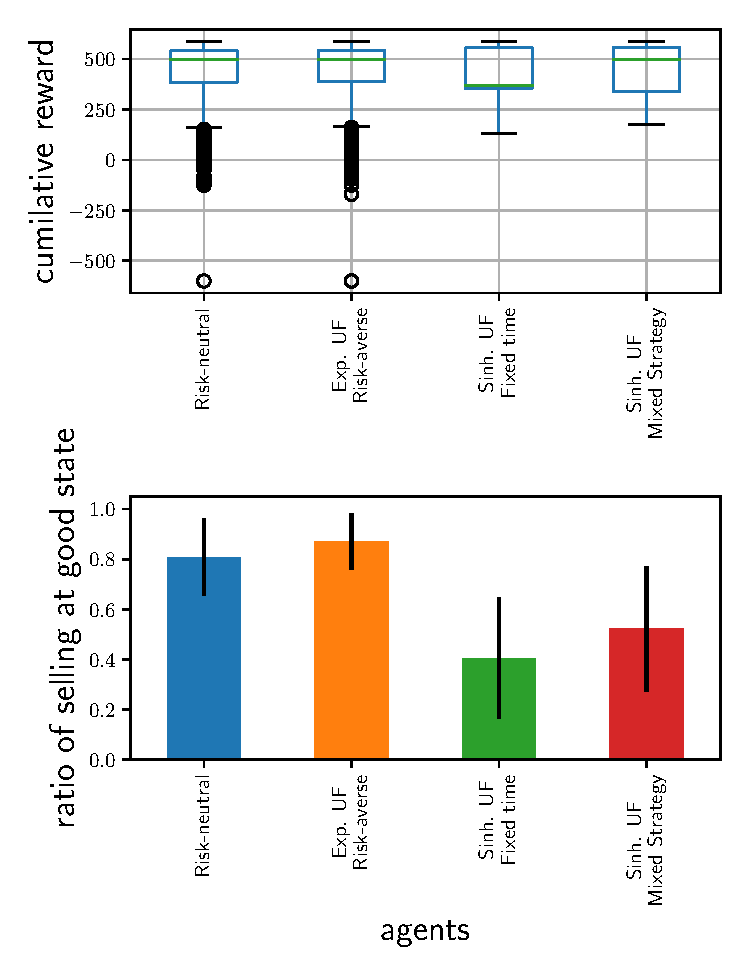
\includegraphics[width=0.99\linewidth]{img/performance.pdf}
    \caption{Accumulated reward and ratio of selling in the good state for reinforcement agents using different utility functions. From left to right: Risk-neutral Agent, Risk-averse agent with exponential UF, Fixed time agent with $\text{sinh}$ UF and mixed stratagy agent with $\text{sinh}$ UF. }\label{fig:perf}
\end{figure}
